\documentclass[a4paper,oneside,reqno]{hmcpset}

\input{../../../../cambridge-macros.tex}

%    Set assignment information here
\newcommand{\authorname}{Feynman Liang, Ambrish Rawat}
\newcommand{\coursename}{MLSALT 6: Information Theory}
\newcommand{\assignmentname}{Assessed Coursework 2}

\name{\authorname}
\class{\coursename}
\assignment{\assignmentname}
\duedate{1/3/2016}

\begin{document}

\title{\coursename\\\assignmentname}
\author{\authorname}
\date{\today}

%\maketitle

\begin{problem}
  Invent a compressor and uncompressor for a source file of $N=10,000$ bits,
  each having probability $f = 0.01$ of being a 1.

  Implement them and estimate how well your method works.
\end{problem}

\begin{solution}
  Our compressor uses a series combination of run-length encoding followed by a
  Huffman symbol code.

  Since the probability of a $0$ ($1-f = 0.99$) is very high, we expect long
  runs of consecutive zeros. Run-length encoding compresses these long runs of
  ``0''s by encoding them as an integer denoting the length of the run. Notice
  that there can be runs of arbitrary length, leading to potentially very many
  symbols after RLE. To handle potentially long sequences, we have a parameter
  $r_{max}$ which limits the length of the longest possible run in RLE. Runs
  exceeding $r_{max}$ are encoded as separate runs, where the first run
  maps to a unique symbol (our implementation uses $r_{max} +1$) denoting
  $r_{max}$ consecutive zeros and the remainder of the run recursively encoded
  in a similar manner. Since both the encoder and decoder know $N=10,000$, we
  can simply zero pad on the decoder and avoid storing the last run.

  For Huffman coding, we initially built the Huffman code based on the
  occurence statistics in the provided file \path{filep.01.10000.txt}.
  While this provides an optimal binary code for compressing this particular file,
  we realized that the code may not perform well on other files generated
  according to the same generative process.

  Fortunately, we know that each bit is generated according to
  $\text{Bernoulli}(f)$. Hence, the run-length $r \sim \text{Geometric}(f)$.
  To construct an optimal binary code for data generated according to this
  process, we can instead use the theoretical occurence probabilities $P(r = k) \propto \begin{cases}
    (1-f)^{k-1}f, &k < r_{max}\\
    (1-f)^{k}, &k = r_{max}
  \end{cases}$ to build the Huffman tree and generate the code.

  Decoding follows this process in reverse. The decoder first uses the same Huffman code
  that was used for encoding to map code words back into run lengths. Runs $r < r_{max}$
  are mapped to $r$ ``0''s followed by a ``1''s and runs $r = r_{max}$ are mapped to
  $r_{max}$ consecutive ``0''s. Since we didn't store the last run on the encoder,
  we zero pad the decoded output until $N=10,000$.

  Our encoder/decoder scheme has two parameters which need to be investigated:
  $r_{max}$ and the occurence statistics used to generate the Huffman trees.
  We investigated the effects of these parameters by plotting the size of the
  compressed \path{filep.01.10000.txt} file while varying these parameters in
  \autoref{fig:size-vs-runLength}

  \begin{figure}[ht!]
    \begin{center}
      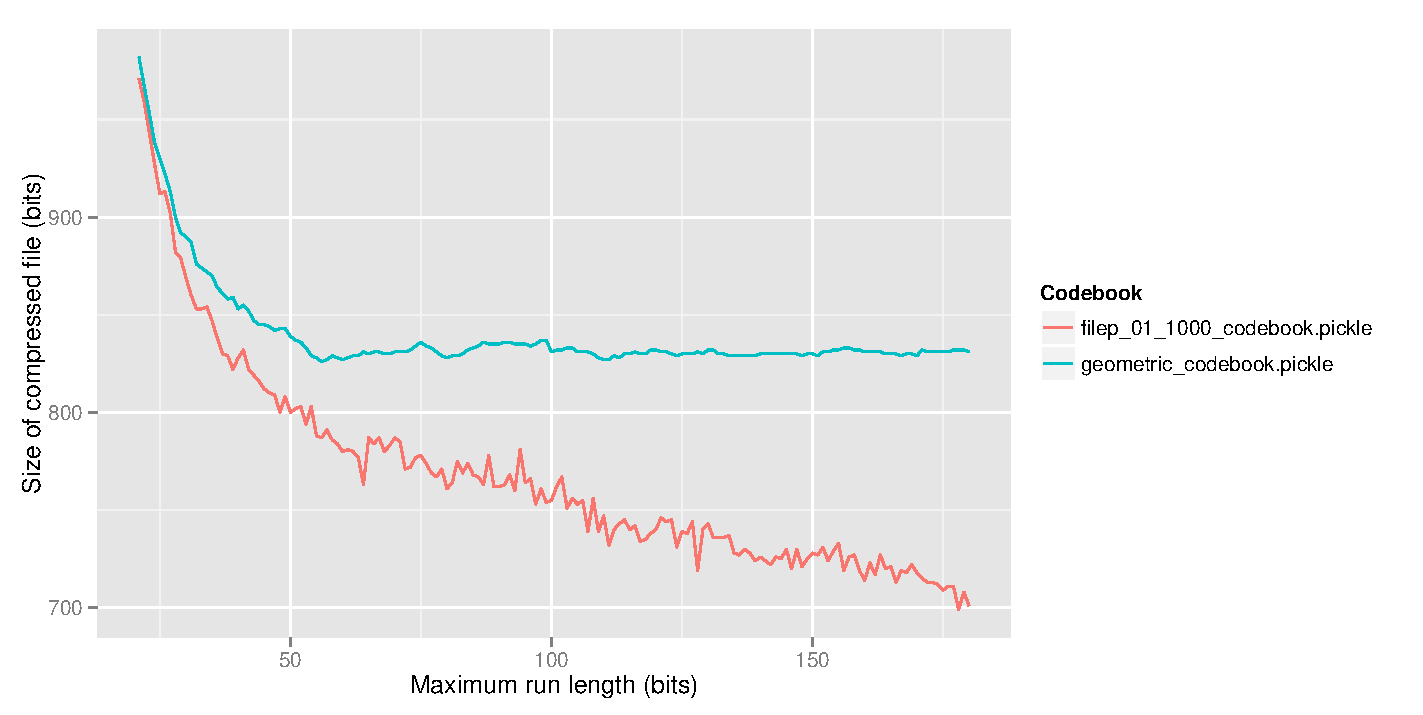
\includegraphics[scale=0.6]{Figures/size-vs-runLength.pdf}
    \end{center}
    \caption{Effect of $r_{max}$ on size of compressed file}
    \label{fig:size-vs-runLength}
  \end{figure}

  The fact that using empirical occurrence statistics from
  \path{filep.01.10000.txt} resulting in smaller files is slightly misleading.
  Since \autoref{fig:size-vs-runLength} plots the results when using
  \path{filep.01.10000.txt} as the file, the code generated from
  \path{filep.01.10000.txt} is the optimal binary code and is expected to
  perform better. However, we would expect it to perform worse on other data
  generated according to $\text{Bernoulli}(f)$ because the statistics in the
  finite sample in \path{filep.01.10000.txt} may not equal the true statistics
  for the generative process. % TODO: show this by syntehsizing other data

  Another interesting trend to note is that increasing $r_{max}$ has the effect
  of decreasing compressed file size up until around $r_{max} \approx 60$,
  after which the compressed file size appears to oscillate with dampening
  amplitude as $r_{max}$ increases. This effect was analyzed in \cite{LoverH},
  where it was shown $r_{max}=69$ (which we follow in our implementation).
  The minimum at $r_{max} \approx 60$ in \autoref{fig:size-vs-runLength} supports
  this analysis, with the difference likely due to the finite sample size
  of \path{filep.01.10000.txt}.

  To understand why, notice if $P(r=r_{max}) \geq 0.5$ then the Huffman
  algorithm will merge $r_{max}$ at the final step (i.e.\ $r_{max}$ will have a
  Huffman code that is one symbol long). Hence, the first bit in a Huffman
  codeword has entropy $H(P(r=r_{max}), 1 - P(r=r_{max}))$. To maximize the
  information content of that bit (and hence minimize the number of bits
  necessary to transmit the same amount of information), we would like a
  uniform distribution i.e.
  \[
    0.5 = P(r=r_{max}) = 0.99^{r_{max}} \implies r_{max} = \frac{\log 0.5}{\log 0.99} \approx 69
  \]
  More generally, because the Huffman tree is a binary tree, the entropy of the
  bit corresponding to the node with $r_{max}$ as a leaf child is maximized
  when $P(r=r_{max})$ is a power of $0.5$, hence $r_{max} \in \{69, 2 \times
  69, 3 \times 69, \cdot\}$ are all possible choices. As $r_{max}$ gets larger,
  this becomes less significant because the probability of $r_{max}$ decreases.

  \subsection{Burrows-Wheeler Transform}

  Inspired by programs like \texttt{bzip}, we also investigated applying a BWT
  to the raw file of bits before compressing. The motivation is that BWT should
  increase the number of long runs of zeros in an invertible manner, allowing
  RLE to provide more compression without any loss of data.



\end{solution}

\bibliographystyle{plain}
\nocite{*} % list all references
\bibliography{refs}

\end{document}
